\usetikzlibrary{arrows.meta, positioning}

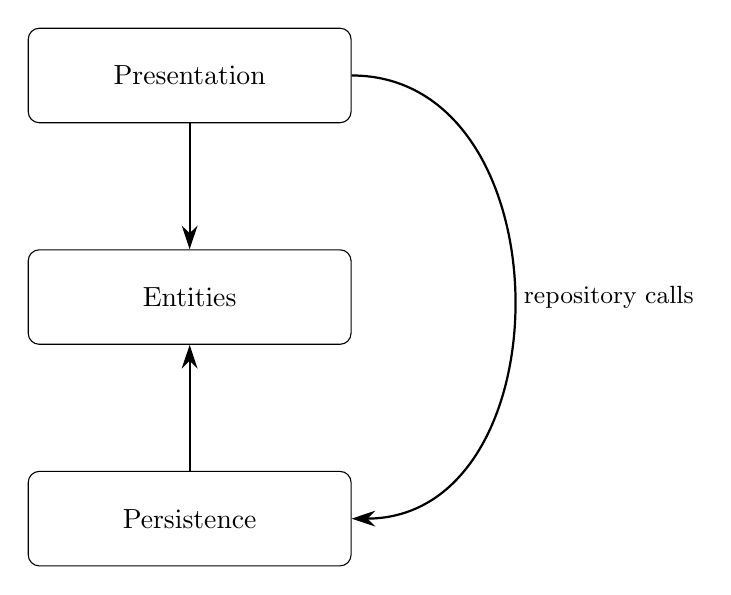
\begin{tikzpicture}[
    node distance=1.6cm and 1.8cm,
    module/.style={draw, rounded corners, minimum width=4.1cm, minimum height=1.2cm, align=center},
    dep/.style={-{Stealth[length=3mm, width=2mm]}, thick}
]
    \node[module] (presentation) {Presentation};
    \node[module, below=of presentation] (entities) {Entities};
    \node[module, below=of entities] (persistence) {Persistence};

    \draw[dep] (presentation.south) -- (entities.north);
    \draw[dep] (presentation.east) to[out=0, in=0, looseness=1.25] node[right, font=\small] {repository calls} (persistence.east);
    \draw[dep] (persistence.north) -- (entities.south);
\end{tikzpicture}
